%This is part of Un soupçon de mathématique sans être agressif pour autant
% Copyright (c) 2012-2013
%   Laurent Claessens, Pauline Klein
% See the file fdl-1.3.txt for copying conditions.

Dans ce chapitres :
\begin{enumerate}
    \item
        Résoudre graphiquement des inéquations : \( f(x)\leq k\) ou \( f(x)\geq g(x)\).
    \item
        Lien tableau de variations, tableau de valeurs et dessin.
    \item
        Comparer des images depuis un tableau de variation.
    \item
        Donner des fonctions sous forme de programmes ou algos.
    \item
        Équation produit.
\end{enumerate}


Les figures \ref{LabelFigFnAffineipcEQfssLabelSubFigFnAffineipcEQf0} et \ref{LabelFigFnAffineipcEQfssLabelSubFigFnAffineipcEQf1} montrent des droites affines. Lorsque \( m>0\), la droite monte; lorsque \( m<0\) elle descend. La pente est d'autant plus forte que \( m\) est grand.
\newcommand{\CaptionFigFnAffineipcEQf}{Deux droites affines.}
\input{Fig_FnAffineipcEQf.pstricks}



\section{Sens de variation d'une fonction}

\subsection{Notion intuitive}

\begin{multicols}{2}

    La fonction ci-contre descend jusqu'à \( -2.5\) puis monte entre \( -2.5\) et \( 2\) pour ensuite descendre.

    Nous disons qu'elle est
    \begin{itemize}
        \item 
            \emph{décroissante} sur \( \mathopen] \infty , -2.5 \mathclose]\);
        \item
            \emph{croissante} sur \( \mathopen[ -2.5 , 2 \mathclose]\);
        \item
            à nouveau décroissante sur \( \mathopen[ 2 , \infty [\).
    \end{itemize}
    
    \columnbreak

%    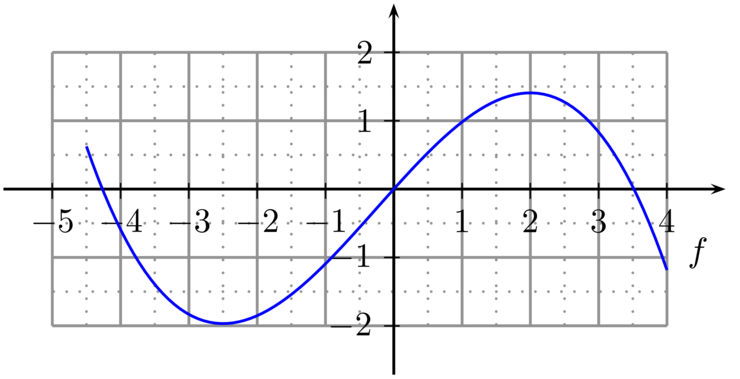
\includegraphics{Picture_FIGLabelFigExVariationRXTkocPICTExVariationRXTkoc-for_eps.pdf}
%The result is on figure \ref{LabelFigExVariationRXTkoc}.
%\newcommand{\CaptionFigExVariationRXTkoc}{<+Type your caption here+>}
\input{Fig_ExVariationRXTkoc.pstricks}

\end{multicols}


\subsection{Définition}

\begin{definition}
      Soit $f$ une fonction définie sur $\defD$ et $I$ un
      intervalle de $\defD$.\\[-2ex]
      \begin{enumerate}
          \item On dit que $f$ est \defe{croissante}{croissante (fonction)} sur $I$
        si et seulement si pour tous réels $a$ et $b$ de $I$, 
        si $a\leq b$ \ alors \ $f(a)\leq f(b)$.
    \item On dit que $f$ est \defe{décroissante}{décroissante (fonction)} sur $I$
        si et seulement si pour tous réels $a$ et $b$ de $I$, 
        si $a\leq b$ \ alors \ $f(a)\geq f(b)$. 
      \end{enumerate}
\end{definition}


\begin{remark}
    Une fonction croissante range les images dans le même ordre que les antécédents. Une fonction décroissante inverse cet ordre. 
\end{remark}


\begin{definition}
    On dit que $f$ est \defe{strictement croissante}{strictement croissante} sur~$I$
  si pour tous réels $a$ et $b$ de $I$ tels que $a<b$, on a $f(a)<f(b)$.

  La fonction \( f\) est \defe{strictement décroissante}{strictement décroissante} sur \( I\) si pour tous réels $a$ et $b$ de $I$ tels que $a<b$, on a $f(a)>f(b)$.
\end{definition}
La différence entre la croissance et la \emph{stricte} croissance est que l'inégalité est stricte.

\begin{definition}
    Soit \( I\) un intervalle de \( \eR\). Nous disons que la fonction \( f\) est \defe{monotone}{monotone} sur $I$ si elle est soit croissante sur $I$, soit décroissante sur $I$.
\end{definition}

\begin{multicols}{2}

    La fonction dessinée ci-contre n'est pas monotone sur l'intervalle \( \mathopen[ -2 , 0 \mathclose]\). Elle est
    \begin{itemize}
        \item 
            monotone décroissante sur \( \mathopen[ -2.5 , -1 \mathclose]\);
        \item
            monotone croissante sur \( \mathopen[ -1 , 1 \mathclose]\);
        \item
            monotone décroissante sur \( \mathopen[ 1 , 1.5 \mathclose]\).
    \end{itemize}

\columnbreak

%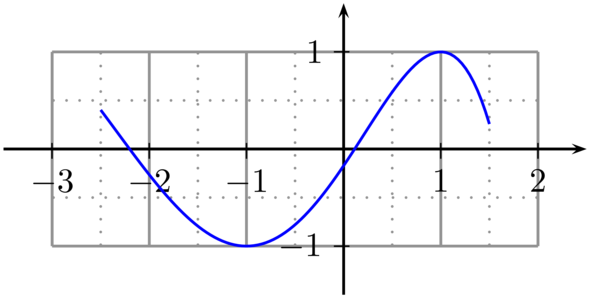
\includegraphics{Picture_FIGLabelFigGrapheVarndvdQMPICTGrapheVarndvdQM-for_eps.pdf}
%The result is on figure \ref{LabelFigGrapheVarndvdQM}.
%\newcommand{\CaptionFigGrapheVarndvdQM}{<+Type your caption here+>}
\input{Fig_GrapheVarndvdQM.pstricks}

\end{multicols}




\begin{definition}
    Soit \( I\) un intervalle. On dit que $f$ est \defe{constante}{constante (fonction)} sur $I$ lorsque pour tous les réels $a$ et $b$ de $I$, on a $f(a)=f(b)$. (Tous les réels de $I$ ont la même image par $f$).
\end{definition}

\begin{multicols}{2}
    Dans ce cas, il existe $k\in\eR$ tel que pour tout $a\in I$, $f(a)=k$. 
    
    La figure ci-contre donne le graphe de la fonction \( f(x)=1.5\) entre \( x=-3\) et \( x=3\).

\columnbreak

%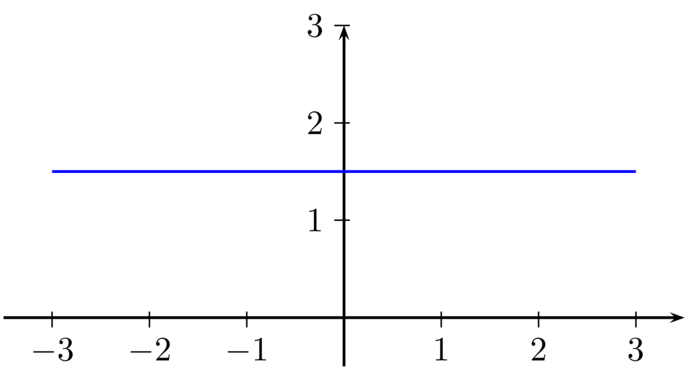
\includegraphics{Picture_FIGLabelFigFoncConstFdDkhWPICTFoncConstFdDkhW-for_eps.pdf}
%The result is on figure \ref{LabelFigFoncConstFdDkhW}.
%\newcommand{\CaptionFigFoncConstFdDkhW}{<+Type your caption here+>}
\input{Fig_FoncConstFdDkhW.pstricks}

\end{multicols}



\begin{wrapfigure}{r}{7.0cm}
   \vspace{-0.5cm}        % à adapter.
   \centering
   \input{Fig_figureCFoZCYe.pstricks}
\end{wrapfigure}

    Sur la figure ci-contre, nous avons tracé les graphes des fonctions données par
    \begin{enumerate}
        \item
            \( f(x)=2x+1\)
        \item
            \( g(x)=2x-2\)
        \item
            \( h(x)=3x-1\)
    \end{enumerate}


Nous constatons que
\begin{enumerate}
    \item
        Les droites représentatives de \( f\) et \( g\) sont parallèles.
    \item
        La droite \( h\) est plus pendue que les deux autres.
\end{enumerate}

